% -----------------------------------------------
% Template for SMC 2021
% Adapted from previous SMC paper templates
% -----------------------------------------------
\documentclass{article}
\usepackage{smc2021}
%%%%%%%%%%%%%%%%%%%%%%%% Some useful packages %%%%%%%%%%%%%%%%%%%%%%%%%%%%%%%
%%%%%%%%%%%%%%%%%%%%%%%% See related documentation %%%%%%%%%%%%%%%%%%%%%%%%%%
\usepackage[caption=false, font=footnotesize]{subfig}% Modern replacement for subfigure package
\usepackage{paralist}% extended list environments
\usepackage[figure,table]{hypcap}% hyperref companion
% Enable for Review only, remove for Camera Ready version
\pagewiselinenumbers


% Use this if english is the only language/alphabet used in the document
\usepackage[english]{babel}


% Title.
% ------
\def\papertitle{Source separation methods for computer-assisted orchestration}

% Authors
% Please note that submissions are NOT anonymous, therefore 
% authors' names have to be VISIBLE in your manuscript. 
% Authors are entered as an ordered list, each one can be linked to multiple affiliations using the correct index.
% Available tags for authors are: \firstname \middlename \lastname \generation \originalname \email \orcid
% Available tags for affiliations are: \unit \department \institution \streetaddress \city \state \postcode \country \type
% type can take as value: University, Company, Music, Independent, Other
%
% \author[]{\mbox{\firstname{}\middlename{}\lastname{}\originalname{}\generation{}\email{}\orcid{}}}
% mbox force an author not to be split over multiple lines
\author[1]{\mbox{\firstname{Luke}\lastname{Dzwonczyk}\email{dz.luke@berkeley.edu}}}
\author[1, 2, 3]{\mbox{\firstname{L\'eo}\lastname{Ch\'edin}}}
\author[1]{\mbox{\firstname{Alejandro}\lastname{Saldarriaga-Fuertes}}}
\author[1]{\mbox{\firstname{Max}\lastname{Sherr}}}
\author[3]{\mbox{\firstname{H\'el\`ene-Camille}\lastname{Crayencour}}}
\author[1]{\mbox{\firstname{Carmine-Emanuele}\lastname{Cella}}}


%%Affiliations
\affil[1]{\department{Center for New Music and Audio Technologies}\institution{University of California, Berkeley}\city{Berkeley}\state{California}\country{USA}\affiliationtype{University}}
\affil[2]{\department{\'Ecole Normale Sup\'erieure Paris-Saclay}\institution{Universi\'e Paris-Saclay}\city{Paris}\state{}\country{France}\affiliationtype{University}}
\affil[3]{\department{Laboratoire des Signaux et Syst\`emes}\institution{Centrale Supélec, CNRS, Université Paris-Saclay}\city{Paris}\state{}\country{France}\affiliationtype{University}}



% Complete setup stage
\completesetup

% Title.
% ------
\title{\papertitle}
% ***************************************** the document starts here ***************
\begin{document}
	%
	\capstartfalse
	\maketitle
	\capstarttrue
	%
	
	\begin{abstract}
		In this paper, we will study the possibility of adding source separation as a pre-processing step to the computer-assisted orchestration process. We first discuss the motivation of this addition and its effects on the quality of orchestrations of multi-layered sounds. Second, we select several state-of-the-art models for both music source separation (separation of instruments) and universal sound separation (separation of arbitrary sounds of different types), and compare their effectiveness for the task of orchestration. We assess which methods best suit the needs of orchestration by applying them on hand picked target sounds, orchestrating the separated outputs, and finally comparing them to the orchestration of the same target without separation. Our experiments show that the quality of orchestrations improves, both qualitatively and quantitatively, indicating that our approach is promising. Finally, we compare unsupervised methods to supervised methods in the case of assisted orchestration, where data is relatively scarce.
	\end{abstract}
	%
	
	\section{Introduction}\label{sec:introduction}
	 
	Computer-assisted composition is a field that focuses on the creation of computational tools to aid in the musical composition process \cite{FerVic2013, Ari2005}. Within this field, target-based computer-assisted musical orchestration is an example of how musical creativity can be assisted and supported by tools such as machine learning. Orchestration has been traditionally taught in an intuitive and non formalized way, and computer-assisted orchestration seeks to help composers by accelerating certain creative processes. In particular, target-based computer-assisted orchestration helps composers explore new timbral possibilities by combining instrumental samples in such a way as to mimic the timbre of a given target sound. Formally, it is the process of creating an orchestral score that best matches an arbitrary target sound given a similarity metric and constraints~\cite{Maresz2003}.
	 
	 Orchidea is a framework and set of tools that is currently considered the state-of-the-art for computer-assisted orchestration. Orchidea embeds the target in a feature space and uses a jointly-optimized multi-objective optimization heuristic and constraint solver to find a combination of samples that best match the target~\cite{Cella18, Cella2020}.
		
	Sound source separation is the process by which a single audio file is separated into multiple sound sources. A perfect separation is able to dissect a sound exactly into its constituent parts, in which each part is an independent sound event. Music source separation is specific application of sound source in which the input audio is expected to be music that is comprised of a subset of instruments or sounds. For example, one music source separation method could attempt to split a song into three parts: voice, bass, and drums. Another aimed at orchestral music may try to separate the input into families of instruments: woodwinds, brass, strings, and percussion. In contrast, universal sound separation does not operate under the assumption that the input is of a musical nature, and can be applied to arbitrary sounds. In this case, the number of sources expected is specified, and the method will attempt to divide the input into the given number of sources.		
		
	Source separation is an important addition to improve orchestration as it allows for the orchestration of more complex sounds in a way that makes sense in an orchestral context. Orchestral music often uses multiple layers, so by separating the layers of a target and individually orchestrating them, the resulting solution is improved. 
		
	For example, consider an example target that has a continuous drone sound throughout and a bird song playing above this drone. Without source separation, Orchidea would detect each note of the bird song as a new onset and cut the target in time at each new note. However, this segmentation in time would also effect the drone, forcing it to have a new onset each time the bird song changes notes. The resulting orchestration would having multiple onsets for the drone, when really only one onset is needed at the beginning of the drone. When source separation is applied to this target, the drone and bird song would be orchestrated separately. Therefore, the drone could be orchestrated by a single onset of note(s) that lasts for the duration of the drone. At the same time, the bird song could have as many new onsets as needed without affecting the drone. The orchestration would be greatly improved by removing the unnecessary onsets in the orchestration of the drone. This is the effect we hope to achieve through implementing source separation in computer-assisted orchestration.
		
	The codebase for this paper can be found at: \url{url needed}, and you can listen to our targets and orchestrations here: \url{url needed}.
		
	
	\section{Methodology}\label{sec:methodology}
	
		
	We compare the effectiveness of different source separation methods for the task of orchestration by applying the separation methods to various targets, orchestrating the separated output of the method, and finally comparing this orchestration to the orchestration of the target if no separation was performed (Fig. \ref{fig:full_diagram}). For example, consider a target sound that is a combination of a low droning sound and high-pitched whistle. With separation, these two sounds would be disentangled into two separate sub-targets and each would be individually orchestrated. The separated orchestrations would then be combined to create the solution. This would then be compared to the orchestration if no separation had been performed.
	
			\begin{figure}[t]
		\centering
			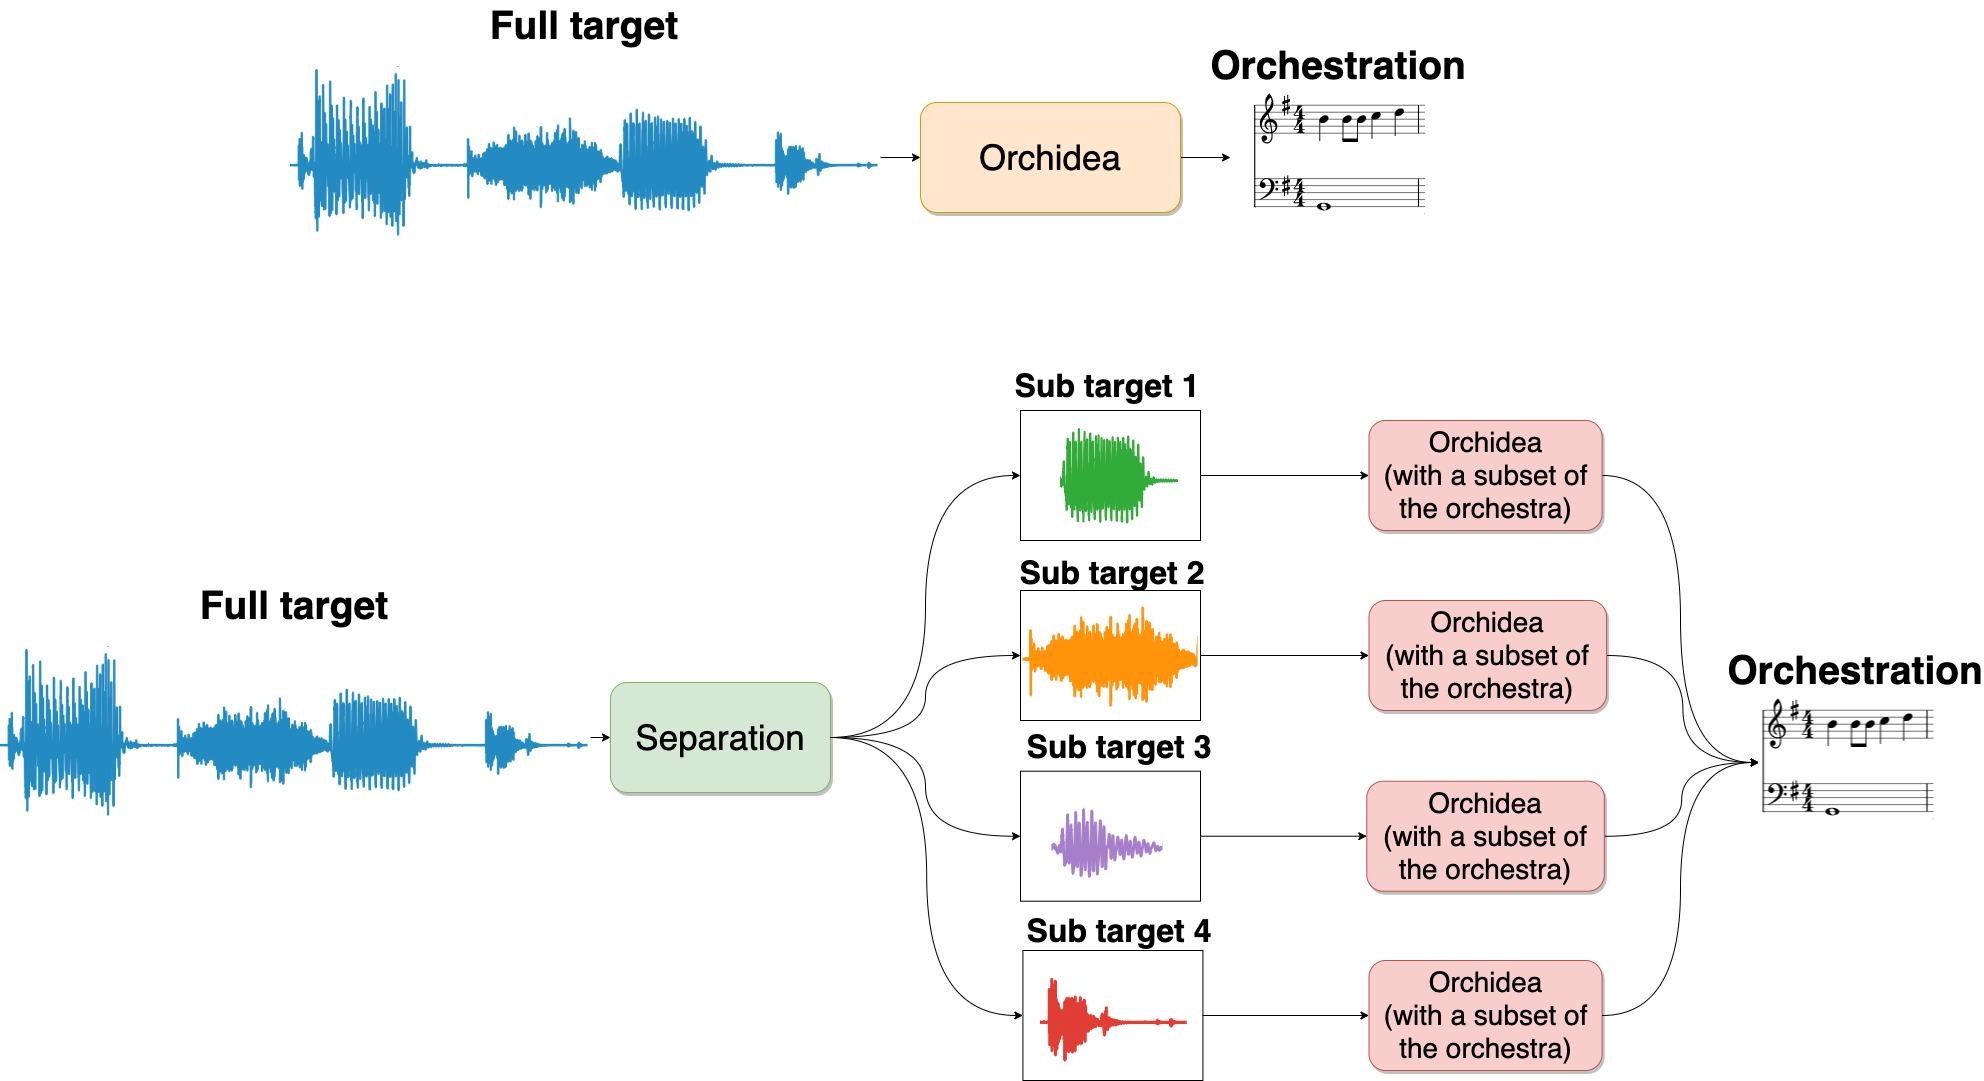
\includegraphics[width=\columnwidth]{figures/diagram.png}
			\caption{Diagram showing the pipeline of the orchestration with (bottom) and without (top) separation. The pipeline using separation divides the target into subtargets that will be orchestrated separately using specific subsets of the orchestra, and then recombined to obtain the full orchestration.}\label{fig:full_diagram}
		\end{figure}
	
	
	
	\section{Experiments}\label{sec:experiments}
	
	We test the effectiveness of five difference source separation methods, both supervised and unsupervised, on 300 custom made targets that are combinations of sounds from different databases. During testing, targets input to each source separation method, which outputs four sub-targets. Then each sub-target is independently orchestrated with a randomly assigned subset of the full orchestra. These orchestrations are then combined to play simultaneously, creating a final orchestrated solution. Then the distance between the target and solution is calculated, giving us a metric to compare the various separation methods.
	
		\subsection{Data}\label{subsec:data}
		We created our own targets as combinations of four source sounds. The sources come from the NIGENS \cite{NIGENS} and BBC \cite{BBC} databases, and freesound.org \cite{freesound}. We selected a total of 90 samples from these databases, choosing sounds that fit the following criteria: 
		
		\begin{enumerate}
			\item Static sounds in which the harmonic average across time is a fitting representation of the sound
			\item Sounds in which there is at least some pitched content and not only noise
		\end{enumerate}			
		The sounds chosen include alarms, bells, engine noises, soundscapes, synthesizer chords, and sound effects. Each target that we used for testing was a combination of four randomly chosen source sounds from the group of 90 sounds. 
		When a target is created, the longest of the four sources is chosen to start playing at the beginning of the target. The other three sources are then randomly assigned different times to begin playing such that they will start between the beginning of the target and half-way through the longest source.
		
		\subsection{Separation Methods}
	
			\subsubsection{Non-negative Matrix Factorization}
			@Max 
			
			
			\subsubsection{OpenUnmix}
			Open-Unmix~\cite{open-unmix} is an open source implementation of a deep music source separation model, based on \cite{Uhlich207}. It is actually composed of multiple models that are trained for each target (such as 'vocals', 'drums', ...). Each of these models is trained on the specific target using the same architecture, based on a three layer bidirectionnal LSTM network. Open-Unmix operates on the Short Time Fourier Transform of the input mixture, which is first standardized. It predicts the target by multiplying the output of the LSTM network with the magnitude spectogram of the input, essentially applying a mask. Open-Unmix also use Wiener filtering as a last processing step.
			
			\subsubsection{Demucs}
			The Demucs~\cite{demucs} architecture is a deep learning model for musical source separation. It takes as input the stereo mixture, and outputs 4 stereo waveforms corresponding to the stems (vocals, bass, drums and other). Demucs is based on a convolutional encoder, a bidirectional LSTM, and a convolutional decoder. The encoder and the decoder are linked with skip U-Net connections. Both the encoder and the decoder are made of 6 blocks, each made of a combination of a convolutional layer with kernel size 8, followed by ReLU activation. Finally there is another convolution with kernel size 1, followed by gated linear units (GLU). The U-network structure allows the decoder to directly access the input signal and to transfer its phase, improving results.	
			
			\subsubsection{ConvTasNet}
			ConvTasNet \cite{tdcn} (TDCN) is a model based on a temporal convolutional encoder-decoder. It uses the audio waveform as input and performs a series of 1-D convolutions at different resolutions with residual connections in order to generate a pool of masks that are then applied on the embedding of the initial waveform to output the separated targets. A final 1-D convolutional layer is used as a decoder to recover the waveforms of each sub target. This type of architecture replaces RNNs in modeling sequential data, as series of dilated convolutions are a good way to capture temporal patterns.
			
			The purpose of the model was initially to separate multiple speakers from a single-channel audio, and was thus trained on speech datasets. Because of its good performance at speech separation, a pre-trained version of the model based on the settings of the paper was added to the benchmark.
			
			\subsubsection{Universal Sound Separation ConvTasNet}
			This version of ConvTasNet, called TDCN++, was improved by \cite{tdcnpp} in order to be used for general sound separation, and not only for speech. The main architecture remains the same as in \cite{tdcn}, and the changes only affected the masking network. More specifically, feature-wise normalization replaces global normalization, residual connection ranges are extended to improve the flow of information, and learnable scale parameters are introduced to weight the outputs of each residual layer. Those modifications help the model to better extract features without drastically increasing its size.
			
			TDCN++ presents the interesting property of having almost the same architecture as TDCN but trained with generic sounds. Thus, it should naturally be better suited for our task, and the comparison between those two models in particular can give good insights about the impact of the data used for training.
	
		\subsection{Testing}
		In order to compare the effectiveness of the separation methods, a full target orchestration and a ground truth orchestration are done for each target. The full target orchestration is the orchestration of the target without any separation performed. The ground truth orchestration takes the four sources that make up the target and orchestrates each one separately, then combines them. This ground truth represents the orchestration that could take place if the separation method was perfect and separated a target exactly into its constituent sources. 
		
		The procedure we used for testing is as follows:
		\begin{enumerate}
			\item The target is created as a combination of four randomly chosen sources, which are offset to begin playing at different times
			\item The full target, without any separation performed, is orchestrated using the entire orchestra
			\item A given separation method is performed on the target, splitting the target into 4 sub-targets
			\item Each sub-target is separately orchestrated using a randomly chosen sub-orchestra that is one quarter the size of the full orchestra, and then each orchestration is combined to play simultaneously
			\item The ground truth orchestration is created by orchestrating the four sources, each with a different sub-orchestra, and then combined to play simultaneously
			\item The distances between target and orchestration are calculated for the full target orchestration, the separated orchestration, and the ground truth orchestration 
		\end{enumerate}	
		
		The orchestrations performed were static orchestrations, meaning a single onset of notes is created for each target, no matter if the target itself has multiple onsets. The OrchideaSOL database of orchestral samples was used with Orchidea to create the orchestrations~\cite{Cella2020c}. This database contains recordings of extended playing techniques, which better fits the often noisy or inharmonic nature of the targets we used. The full orchestra, of which non-overlapping subsets were selected to orchestrate the subtargets, contained the following instruments: 8 violins, 4 violas, 3 cellos, 1 bass, 2 oboes, 2 flutes, 2 clarinets in B$\flat$, 2 bassoons, 2 trumpets, 2 trombones, and 2 French horns.
		
		\begin{figure}[t]
		\centering
			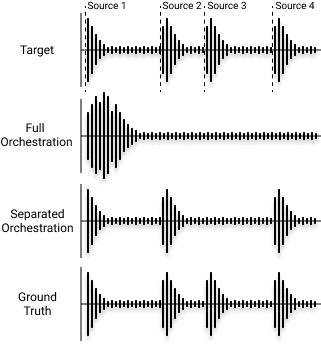
\includegraphics[width=\columnwidth]{figures/orch.jpg}
			\caption{Example waveforms showing onsets of the four sources in the target, and possible onsets in the full, separated, and ground truth orchestrations. In this example, the separation method could not distinguish between sources 2 and 3 and identified them as a single sub-target. Therefore, the separated orchestration has only 3 onsets, one of them being an orchestration that combines sources 2 and 3. Note that this is a simplified representation, in the actual targets sources overlap in time and are not as discrete as this diagram shows.}\label{fig:orchestrations}
		\end{figure}		
		
		As described in Section \ref{subsec:data}, each target is comprised of four sources that are offset in time to begin playing at different times. Figure \ref{fig:orchestrations} illustrates the effect this offset has on the full target, separated, and ground truth orchestrations. The full target orchestration places all onsets at the beginning of the orchestration, since it is unable to differentiate between different sources, it cannot place the different orchestrations at the appropriate offsets. However, the separated orchestrations are able to correctly place the onsets of the sub-target orchestrations so far as the method has correctly separated out the sources. In the ground truth orchestration, the sources are offset by the same amount as they are in the creation of the target, leading to the ground truth having each source orchestration beginning at the correct time.
		
		\subsection{Evaluation}
		We compare the effectiveness of different separation methods by comparing how well they work for orchestration. The output of a method is orchestrated, and these orchestrations are compared. A quantitative evaluation is performed through the use of a distance metric that measures the spectral distance between target and solution. 
		
		The distance metric cuts the target and solution into successive frames that are 4,000 samples in length, then calculates the spectral distance as defined in Eqn. \ref{eqn:distance} between corresponding frames. The spectral distance metric is proposed in \cite{Cella2020} as part of the cost function used in Orchidea during the optimization, and used in \cite{Cella2020b} to compare accuracies of orchestrations. The equation takes in the full FFT of the target $x$ and full FFT of the solution $\tilde{x}$. Then for each bin $k$ of the FFT, it calculates the absolute difference between the values. The differing values of $\lambda_1$ and $\lambda_2$ allow the metric to penalize the solution in different ways. For our purposes, we used $\lambda_1 = 0.5$ and $\lambda_2 = 10$, which penalizes a solution that overshoots the harmonic energy of the target.
		
		\begin{equation}\label{eqn:distance}
d(x, \tilde{x}) =\lambda_1 \sum_k \delta_{k1}(x_k - \tilde{x}_k) + \lambda_2 \sum_k \delta_{k2}|x_k - \tilde{x	}_k| \\
\end{equation}
where $\delta_{k1} = 1 \text{  if  } x_k \ge \tilde{x}_k, 0 \text{  otherwise}$; and $\delta_{k2} = 1 \text{  if  } x_k < \tilde{x}_k, 0 \text{  otherwise}$.
	
	
	\begin{table}[t]
		\begin{center}
			\begin{tabular}{|c|c|}
				\hline
				& Average distance \\
				\hline
				Full target & 24.96 \\
				\hline
				NMF & 22.44 \\
				\hline
				Demucs & 25.11 \\
				\hline
				OpenUnmix & 24.48\\
				\hline
				TDCN & 26.44\\
				\hline
				TDCN++ & 24.38 \\
				\hline
				Ground truth & 24.19 \\
				\hline
			\end{tabular}
		\end{center}
		\caption{Average across 300 targets showing the distance between target and orchestration for various methods. "Full target" means no separation was performed.}
		\label{tab:distances}
	\end{table}
		
		\subsection{Results}
		The average distances for full target, separated, and ground truth orchestrations are displayed in Table \ref{tab:distances}. These results are the average distance between target and orchestration for 300 different targets. We found that NMF performed the best out of all separation methods, and even outperformed the ground truth orchestrations. TDCN++, OpenUnmix, and NMF performed better than the full target orchestrations, meaning that separating targets using these methods leads to a better orchestration than if no separation is applied.
	
	\section{Conclusions}\label{sec:conclusions}
	In this paper, we addressed the problem of using source separation as a pre-processing step for computer-assisted orchestration. The results show that performing source separation followed by a static orchestration of each individual sub-target improved the spectral distance between the original target and its orchestrated version in three out of five of the methods tested.
	
	Furthermore, the one unsupervised method we tested, NMF, outperformed all the supervised methods. It is important to notice that for the supervised methods, we used pre-trained versions of the neural models. All of these models, except for TDCN++, were trained on musical data. However, we tested them on a wide range of targets, many of which were not strictly musical. This could explain why Demucs, OpenUnmix, and TDCN performed worse than NMF, and why TDCN++, which was trained on arbitrary sounds, outperformed the other supervised methods. Therefore, we may infer from our results that models trained on generic sounds generate a better separation for orchestration when compared to models trained only on musical sounds.
	
	Since unsupervised methods perform well, it is reasonable to think that supervised methods trained on a dataset of arbitrary sounds could yield better overall performance for orchestration.
	
	\section{Future Work}\label{sec:futurework}

	As we stated in Section \ref{sec:conclusions}, we believe that one of the reasons the supervised methods did not perform as well is because of the data they were trained on. Therefore, a natural next step is to train these models ourselves with sounds that are more applicable to computer-assisted orchestration.
	
	Another aspect we would like to work on is the assignment of the orchestras. Currently, the subset of the orchestra that is assigned to each sub-target is randomly selected. However, it is possible that this random assignment could reduce the quality of the final orchestration. If, for example, one of the sub-targets contains mostly low pitch content, but the orchestra assigned to it contains mostly violins, violas, flutes, and oboes, the resulting orchestration will suffer. To solve this problem, a step could be added that jointly-optimizes the the orchestras assigned to each sub-target, ultimately choosing an assignment that leads to the best orchestration of each sub-target.
	
	Finally, one or multiple of the separation methods we tested should be implemented in Orchidea in order to improve the orchestrations Orchidea is capable of creating. NMF performed the best across the targets we tested on, and therefore makes sense to be added to Orchidea. However, it could also make sense to add one of the musical source spearation methods, such as OpenUnmix, to allow users to choose different methods based on the targets they are orchestrating.
	
	\begin{acknowledgments}
		At the end of the Conclusions, acknowledgements to people, projects, funding agencies, etc. can be included after the second-level heading  ``Acknowledgments'' (with no numbering).
	\end{acknowledgments} 
	
	%%%%%%%%%%%%%%%%%%%%%%%%%%%%%%%%%%%%%%%%%%%%%%%%%%%%%%%%%%%%%%%%%%%%%%%%%%%%%
	%bibliography here
	\bibliography{references}
	
\end{document}
